% Artigo no modelo SBC (sbc-template.sty), com citacoes e referencias segundo a ABNT
% (NBR 10520 e NBR 6023, pacote abnTeX2). Compilar com: tectonic artigo.tex
\documentclass[12pt]{article}

\usepackage{sbc-template}
\usepackage[T1]{fontenc}
\usepackage[utf8]{inputenc}
\usepackage[brazil]{babel}
\usepackage{graphicx}
\usepackage{booktabs}
\usepackage{amsmath}
\usepackage[colorlinks=true,urlcolor=blue,linkcolor=black,citecolor=black]{hyperref}
\usepackage[alf]{abntex2cite}
\providecommand{\htmladdnormallink}[2]{\href{#2}{#1}}

% ABNT: "Figura 1 -- Titulo", secoes numeradas sem ponto final e titulo "REFERENCIAS"
\renewcommand{\captionlabeldelim}{~--}
\titlelabel{\thetitle\hspace{1ex}}
\addto\captionsbrazil{\renewcommand{\refname}{REFERÊNCIAS}}

\newcommand{\repo}{\url{https://github.com/Player07x/manet-routing-ns3}}

\sloppy

\title{Impacto da mobilidade no desempenho dos protocolos AODV, OLSR e DSDV em redes MANET: um experimento reprodutível no ns-3}

\author{João Antonio André Barbosa Camilo\inst{1}, João Pedro Neto\inst{1}}

\address{Instituto Federal de Educação, Ciência e Tecnologia de Goiás (IFG)\\
  Câmpus Inhumas -- Inhumas -- GO -- Brasil
  \email{joaoantoniobr07@gmail.com, jpns.max@gmail.com}
}

\begin{document}

\maketitle

\begin{resumo}
Este artigo avalia como a velocidade dos nós afeta os protocolos de roteamento AODV, OLSR e DSDV em uma MANET simulada no ns-3.48: 20 nós em 500 $\times$ 500 m, mobilidade \textit{Random Waypoint} de 1 a 20 m/s, quatro fluxos UDP e 120 s, com uma extensão em 750 $\times$ 750 m (480 execuções, 20 repetições por combinação, intervalos de confiança de 95\%). A entrega caiu com a velocidade nos três protocolos; a 20 m/s em 500 $\times$ 500 m, o PDR foi de 92,5\% no AODV, 79,5\% no OLSR e 74,6\% no DSDV, que perderam mais pacotes ao usar vizinhos já fora do alcance. O OLSR teve o menor atraso. O ARP padrão do ns-3.48 distorcia a comparação e foi neutralizado.

\textbf{Palavras-chave:} MANET; AODV; OLSR; DSDV; ns-3; mobilidade.
\end{resumo}

\begin{abstract}
This paper evaluates how node speed affects the AODV, OLSR and DSDV routing protocols in a MANET simulated in ns-3.48: 20 nodes in 500 $\times$ 500 m, Random Waypoint mobility from 1 to 20 m/s, four UDP flows and 120 s, with an extension in 750 $\times$ 750 m (480 runs, 20 replications per combination, 95\% confidence intervals). Delivery decreased with speed for all protocols; at 20 m/s in 500 $\times$ 500 m, PDR was 92.5\% for AODV, 79.5\% for OLSR and 74.6\% for DSDV, which lost more packets by using neighbors already out of range. OLSR had the lowest delay. The default ARP of ns-3.48 distorted the comparison and was neutralized.

\textbf{Keywords:} MANET; AODV; OLSR; DSDV; ns-3; mobility.
\end{abstract}

\begin{center}
\fbox{\parbox{0.9\textwidth}{\centering
\textbf{Repositório público com código, dados e instruções de reprodução:}\\
\repo\\
\small Versão correspondente a este artigo: \textit{tag} \texttt{artigo-v1}}}
\end{center}

\section{INTRODUÇÃO}

Em uma rede móvel \textit{ad hoc} (MANET), os nós se comunicam sem infraestrutura e encaminham pacotes uns dos outros por múltiplos saltos. Como os nós se movem, enlaces surgem e desaparecem, e o roteamento precisa reagir: protocolos reativos, como o AODV, buscam rotas apenas quando há dados a enviar, enquanto protocolos proativos, como o OLSR e o DSDV, mantêm rotas atualizadas continuamente \cite{rfc3561,rfc3626,perkins1994}. Estudos clássicos mostram que o desempenho relativo dessas estratégias depende do cenário e, em particular, da mobilidade \cite{broch1998,das2000}.

Este trabalho responde à pergunta: \textit{como diferentes níveis de mobilidade afetam o desempenho dos protocolos AODV, OLSR e DSDV em uma rede MANET?} Para isso, realiza-se no ns-3 um experimento controlado em que apenas a velocidade e o protocolo variam, além de uma extensão com menor densidade de nós. Como estudos de MANET por simulação frequentemente não permitem reprodução \cite{kurkowski2005}, código, dados e instruções estão no repositório indicado acima.

\section{FUNDAMENTAÇÃO TEÓRICA}

O \textbf{AODV} descobre rotas sob demanda, por pedidos (RREQ) difundidos na rede e respostas (RREP) pelo caminho reverso; quando um enlace se rompe, uma mensagem de erro (RERR) invalida a rota e provoca nova descoberta \cite{rfc3561}. No ns-3.48, a quebra é detectada pela perda de dois HELLOs (enviados a cada 1 s) ou por falha informada pela camada MAC, e os pacotes sem rota aguardam em um \textit{buffer} de até 64 pacotes por 30 s \cite{ns3modelos}. O \textbf{OLSR} é proativo e baseado em estado de enlace: HELLOs a cada 2 s descobrem vizinhos e elegem os \textit{multipoint relays} (MPR), únicos nós que retransmitem as mensagens de topologia (TC, a cada 5 s) \cite{rfc3626}; no ns-3, um vizinho só é descartado 6 s após o último HELLO, avisos da camada MAC não são usados e pacotes sem rota são descartados na origem. O \textbf{DSDV} é proativo e baseado em vetor de distância, com números de sequência emitidos pelo destino para distinguir rotas novas de obsoletas \cite{perkins1994}; no ns-3, cada nó envia a tabela completa a cada 15 s, além de atualizações disparadas por mudanças, remove rotas após 45 s sem atualização e guarda até 5 pacotes por destino enquanto não há rota \cite{ns3modelos}. A mobilidade segue o \textit{Random Waypoint}, em que cada nó vai em linha reta até um destino aleatório e pausa antes de escolher o próximo \cite{camp2002}, e as métricas são coletadas pelo FlowMonitor \cite{carneiro2009}.

\section{METODOLOGIA}

Um único programa (\texttt{src/manet-routing.cc}) recebe protocolo, área, velocidade e repetição como parâmetros de linha de comando; a Tabela~\ref{tab:parametros} resume o cenário. Na matriz-base (500 $\times$ 500 m) apenas a velocidade e o protocolo variam; a extensão do grupo repete a matriz em 750 $\times$ 750 m, reduzindo a densidade de 80 para cerca de 36 nós/km$^2$.

\begin{table}[ht]
\centering
\caption{Parâmetros do experimento}
\label{tab:parametros}
\small
\begin{tabular}{@{}ll@{}}
\toprule
\textbf{Parâmetro} & \textbf{Valor} \\
\midrule
Simulador & ns-3.48 (Ubuntu 26.04.1 LTS, g++ 15.2.0) \\
Enlace e canal & IEEE 802.11b \textit{ad hoc}; alcance fixo de 250 m (modelo de disco) \\
Nós e área & 20 nós; 500 $\times$ 500 m (base) e 750 $\times$ 750 m (extensão) \\
Mobilidade & \textit{Random Waypoint}; 1, 5, 10 e 20 m/s constantes; pausa de 1 s \\
Tráfego & 4 fluxos UDP (nó $i \rightarrow$ nó $19-i$), 512 B a 1 pacote/s, de 10 s a 120 s \\
Protocolos & AODV, OLSR e DSDV com os parâmetros padrão do ns-3.48 \\
Repetições & 20 por combinação (\textit{seed} 1, \textit{run} 1 a 20): 480 execuções de 120 s \\
\bottomrule
\end{tabular}

\footnotesize Fonte: elaborada pelos autores (2026).
\end{table}

\textbf{Rádio e ARP.} O canal padrão do ns-3.48 (802.11ax, perda \textit{log-distance}, limiar de preâmbulo de $-82$~dBm) alcança cerca de 51 m, o que particionaria a área de 500 $\times$ 500 m; adotou-se o alcance nominal de 250 m usado por \citeonline{broch1998}, com o modelo \texttt{RangePropagationLossModel}. Na validação, o ARP padrão do ns-3.48 mostrou-se um artefato: as retransmissões de requisição ocorrem a cada 1 s exato, sem variação aleatória, de modo que requisições de vizinhos iniciadas no mesmo instante colidem em todas as tentativas e o vizinho é considerado inalcançável por 100 s. Com ele, na repetição 20 em 750 $\times$ 750 m a 1 m/s, três fluxos do AODV entregaram 0\%, 0\% e 4,5\% dos pacotes, enquanto OLSR e DSDV, com as mesmas trajetórias, entregaram mais de 80\%. As tabelas ARP foram, então, pré-preenchidas com entradas permanentes; o pré-preenchimento automático do ns-3 (\texttt{NeighborCacheHelper}) não serve, porque o AODV ignora entradas desse tipo e deixa de detectar enlaces quebrados. O comportamento original pode ser reproduzido com \texttt{--arp=dinamico}.

\textbf{Tráfego, repetições e métricas.} Cada cliente UDP começa com um atraso aleatório de até 1 s, para que os fluxos não transmitam sempre no mesmo instante, e as respostas do \textit{echo} não entram nas métricas. Com \textit{seed} fixa, o \textit{run} identifica a repetição; para a mesma repetição, as trajetórias dos nós são idênticas nos três protocolos, o que torna a comparação pareada. Por execução, calcula-se: PDR $=$ recebidos $/$ transmitidos pela aplicação $\times 100$; \textit{throughput} $=$ bytes recebidos $\times 8 /$ 110 s (de 10 s a 120 s); atraso $=$ \texttt{delaySum} $/$ recebidos; e \textit{jitter} $=$ \texttt{jitterSum} $/$ (recebidos $-1$), por fluxo. Os bytes incluem os cabeçalhos IP e UDP, e a carga ofertada é de 0,01728 Mbps. Como apoio à discussão, registram-se a mediana e o percentil 95 do atraso (histograma do FlowMonitor) e os quadros descartados pela camada MAC ao esgotar as retransmissões, que indicam envio a um vizinho fora do alcance. Os resultados são médias de 20 repetições com intervalo de confiança (IC) de 95\% pela distribuição \textit{t} de Student \cite{pawlikowski2002}.

\section{RESULTADOS E DISCUSSÃO}

\begin{figure}[ht]
\centering
\caption{Métricas em função da velocidade no cenário-base (a--d) e na extensão (e--h)}
\label{fig:resultados}
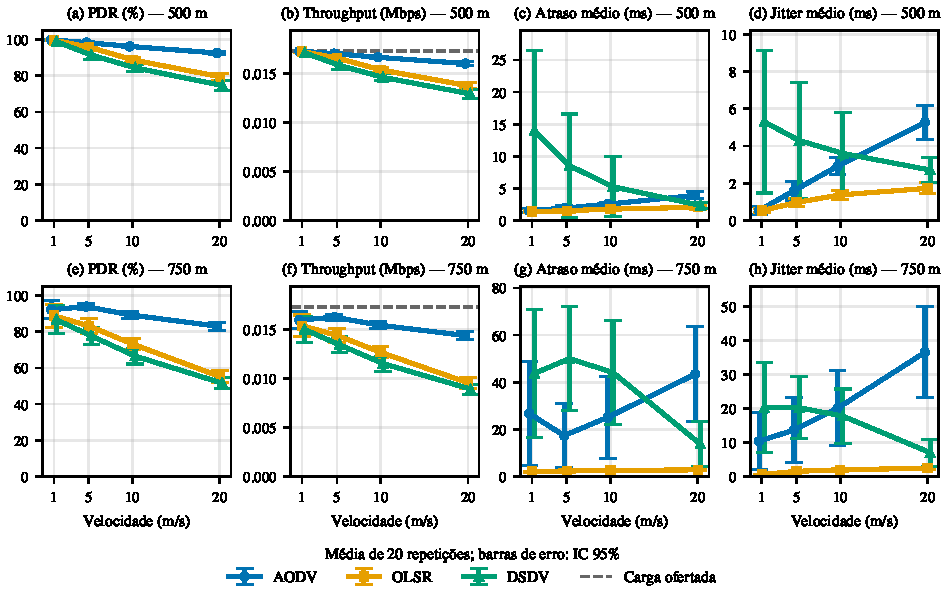
\includegraphics[width=\textwidth]{figuras/metricas_artigo.pdf}\\
\footnotesize Fonte: elaborada pelos autores (2026), a partir de \texttt{data/processed/resultados-agregados.csv}.
\end{figure}

\textbf{Cenário-base.} Nos três protocolos, a entrega cai com a velocidade (Figura~\ref{fig:resultados}a): entre 1 e 20 m/s, o PDR do AODV passa de 99,8\% para 92,5\%, o do OLSR de 99,6\% para 79,5\% e o do DSDV de 98,8\% para 74,6\%. A 1 m/s as diferenças não passam de 1 ponto percentual (p.p.); a partir de 5 m/s, a diferença pareada entre cada par de protocolos é positiva, com IC 95\% que não inclui zero (AODV $-$ OLSR $=$ 13,1 $\pm$ 1,2 p.p. a 20 m/s). Como a carga é fixa e muito menor que a capacidade do enlace, o \textit{throughput} reproduz o PDR (Figura~\ref{fig:resultados}b). A ordem é explicada pelos descartes na camada MAC: a partir de 5 m/s, de 85\% a 100\% das perdas ocorreram após esgotar as retransmissões, ou seja, em envios a vizinhos que já haviam saído do alcance, atingindo, a 20 m/s, 25,4\% dos pacotes do DSDV, 20,2\% do OLSR e 6,6\% do AODV. Isso é compatível com o modo como cada protocolo percebe a quebra: o AODV é avisado pela camada MAC e repara a rota, o OLSR mantém o vizinho por até 6 s e o DSDV espera uma atualização com número de sequência novo. O resultado concorda com \citeonline{broch1998}, em que o DSDV foi o mais sensível à mobilidade.

O atraso e o \textit{jitter} (Figura~\ref{fig:resultados}c--d) revelam o compromisso oposto. No cenário-base, a mediana do atraso por execução fica, em média, entre 0,65 e 1,02 ms, perto do tempo de envio de um quadro de 576 B a 11 Mb/s em um salto (cerca de 0,66 ms); as diferenças entre as médias vêm de poucos pacotes muito atrasados. O OLSR tem o menor atraso médio (1,39 a 2,07 ms) porque não armazena pacotes sem rota. O do AODV cresce com a velocidade (1,53 a 3,92 ms; percentil 95 de 20,9 ms a 20 m/s), pois os pacotes aguardam no \textit{buffer} a cada nova descoberta de rota. No DSDV, a média alta e variável a 1 m/s (14,0 $\pm$ 12,4 ms) vem do início de algumas repetições: no registro por pacote da repetição 9, os pacotes de um fluxo enviados entre 10 e 14 s esperaram de 6,4 a 10,3 s até o DSDV aprender a rota, por volta de 20 s de simulação; depois disso, os maiores atrasos (de 95 a 191 ms) ocorreram a cada 15 s, o período das atualizações completas. Trata-se da convergência inicial do protocolo, e não de efeito da mobilidade.

\textbf{Extensão.} Com os mesmos 20 nós em uma área 2,25 vezes maior (Figura~\ref{fig:resultados}e--h), todos entregam menos e a vantagem do AODV aumenta: a 20 m/s, o PDR é de 83,1\% no AODV, 55,3\% no OLSR e 51,6\% no DSDV, e a diferença pareada AODV $-$ OLSR sobe para 27,8 $\pm$ 2,1 p.p. Os descartes na camada MAC chegam a 48,4\% dos pacotes do DSDV e 36,8\% do OLSR. Com menos vizinhos, a rede também se divide: o OLSR descartou na origem, por falta de rota, de 5,3\% a 9,7\% dos pacotes, e na repetição 17 a 1 m/s um fluxo não entregou nenhum pacote em nenhum protocolo, o que alarga os intervalos a 1 m/s. O custo da entrega do AODV é o atraso, que chega a 43,4 ms a 20 m/s, enquanto o OLSR fica abaixo de 3 ms. A extensão confirma e acentua a tendência do cenário-base.

\section{CONCLUSÃO}

Nas condições simuladas, o aumento da velocidade reduziu a entrega dos três protocolos, e a queda foi menor no AODV, que manteve PDR de pelo menos 92,5\% em 500 $\times$ 500 m e 83,1\% em 750 $\times$ 750 m. Os protocolos proativos perderam mais pacotes por continuarem usando vizinhos que já haviam saído do alcance, efeito que cresce com a velocidade e com a menor densidade. Em contrapartida, o OLSR teve os menores atraso e \textit{jitter} médios, e o atraso do AODV aumentou com a mobilidade; a escolha depende da métrica prioritária para a aplicação. As conclusões valem para o cenário estudado: alcance fixo sem desvanecimento, carga leve, parâmetros padrão do ns-3.48, tabelas ARP pré-preenchidas e posições iniciais uniformes. O estudo também mostrou que detalhes da pilha simulada, como o ARP, podem dominar a comparação se não forem verificados. Trabalhos futuros podem usar propagação realista, cargas maiores e outros temporizadores para o OLSR e o DSDV.

\bibliography{referencias}

\end{document}
